% Options for packages loaded elsewhere
\PassOptionsToPackage{unicode}{hyperref}
\PassOptionsToPackage{hyphens}{url}
%
\documentclass[
]{article}
\usepackage{amsmath,amssymb}
\usepackage{lmodern}
\usepackage{iftex}
\ifPDFTeX
  \usepackage[T1]{fontenc}
  \usepackage[utf8]{inputenc}
  \usepackage{textcomp} % provide euro and other symbols
\else % if luatex or xetex
  \usepackage{unicode-math}
  \defaultfontfeatures{Scale=MatchLowercase}
  \defaultfontfeatures[\rmfamily]{Ligatures=TeX,Scale=1}
\fi
% Use upquote if available, for straight quotes in verbatim environments
\IfFileExists{upquote.sty}{\usepackage{upquote}}{}
\IfFileExists{microtype.sty}{% use microtype if available
  \usepackage[]{microtype}
  \UseMicrotypeSet[protrusion]{basicmath} % disable protrusion for tt fonts
}{}
\makeatletter
\@ifundefined{KOMAClassName}{% if non-KOMA class
  \IfFileExists{parskip.sty}{%
    \usepackage{parskip}
  }{% else
    \setlength{\parindent}{0pt}
    \setlength{\parskip}{6pt plus 2pt minus 1pt}}
}{% if KOMA class
  \KOMAoptions{parskip=half}}
\makeatother
\usepackage{xcolor}
\usepackage[margin=1in]{geometry}
\usepackage{color}
\usepackage{fancyvrb}
\newcommand{\VerbBar}{|}
\newcommand{\VERB}{\Verb[commandchars=\\\{\}]}
\DefineVerbatimEnvironment{Highlighting}{Verbatim}{commandchars=\\\{\}}
% Add ',fontsize=\small' for more characters per line
\usepackage{framed}
\definecolor{shadecolor}{RGB}{248,248,248}
\newenvironment{Shaded}{\begin{snugshade}}{\end{snugshade}}
\newcommand{\AlertTok}[1]{\textcolor[rgb]{0.94,0.16,0.16}{#1}}
\newcommand{\AnnotationTok}[1]{\textcolor[rgb]{0.56,0.35,0.01}{\textbf{\textit{#1}}}}
\newcommand{\AttributeTok}[1]{\textcolor[rgb]{0.77,0.63,0.00}{#1}}
\newcommand{\BaseNTok}[1]{\textcolor[rgb]{0.00,0.00,0.81}{#1}}
\newcommand{\BuiltInTok}[1]{#1}
\newcommand{\CharTok}[1]{\textcolor[rgb]{0.31,0.60,0.02}{#1}}
\newcommand{\CommentTok}[1]{\textcolor[rgb]{0.56,0.35,0.01}{\textit{#1}}}
\newcommand{\CommentVarTok}[1]{\textcolor[rgb]{0.56,0.35,0.01}{\textbf{\textit{#1}}}}
\newcommand{\ConstantTok}[1]{\textcolor[rgb]{0.00,0.00,0.00}{#1}}
\newcommand{\ControlFlowTok}[1]{\textcolor[rgb]{0.13,0.29,0.53}{\textbf{#1}}}
\newcommand{\DataTypeTok}[1]{\textcolor[rgb]{0.13,0.29,0.53}{#1}}
\newcommand{\DecValTok}[1]{\textcolor[rgb]{0.00,0.00,0.81}{#1}}
\newcommand{\DocumentationTok}[1]{\textcolor[rgb]{0.56,0.35,0.01}{\textbf{\textit{#1}}}}
\newcommand{\ErrorTok}[1]{\textcolor[rgb]{0.64,0.00,0.00}{\textbf{#1}}}
\newcommand{\ExtensionTok}[1]{#1}
\newcommand{\FloatTok}[1]{\textcolor[rgb]{0.00,0.00,0.81}{#1}}
\newcommand{\FunctionTok}[1]{\textcolor[rgb]{0.00,0.00,0.00}{#1}}
\newcommand{\ImportTok}[1]{#1}
\newcommand{\InformationTok}[1]{\textcolor[rgb]{0.56,0.35,0.01}{\textbf{\textit{#1}}}}
\newcommand{\KeywordTok}[1]{\textcolor[rgb]{0.13,0.29,0.53}{\textbf{#1}}}
\newcommand{\NormalTok}[1]{#1}
\newcommand{\OperatorTok}[1]{\textcolor[rgb]{0.81,0.36,0.00}{\textbf{#1}}}
\newcommand{\OtherTok}[1]{\textcolor[rgb]{0.56,0.35,0.01}{#1}}
\newcommand{\PreprocessorTok}[1]{\textcolor[rgb]{0.56,0.35,0.01}{\textit{#1}}}
\newcommand{\RegionMarkerTok}[1]{#1}
\newcommand{\SpecialCharTok}[1]{\textcolor[rgb]{0.00,0.00,0.00}{#1}}
\newcommand{\SpecialStringTok}[1]{\textcolor[rgb]{0.31,0.60,0.02}{#1}}
\newcommand{\StringTok}[1]{\textcolor[rgb]{0.31,0.60,0.02}{#1}}
\newcommand{\VariableTok}[1]{\textcolor[rgb]{0.00,0.00,0.00}{#1}}
\newcommand{\VerbatimStringTok}[1]{\textcolor[rgb]{0.31,0.60,0.02}{#1}}
\newcommand{\WarningTok}[1]{\textcolor[rgb]{0.56,0.35,0.01}{\textbf{\textit{#1}}}}
\usepackage{graphicx}
\makeatletter
\def\maxwidth{\ifdim\Gin@nat@width>\linewidth\linewidth\else\Gin@nat@width\fi}
\def\maxheight{\ifdim\Gin@nat@height>\textheight\textheight\else\Gin@nat@height\fi}
\makeatother
% Scale images if necessary, so that they will not overflow the page
% margins by default, and it is still possible to overwrite the defaults
% using explicit options in \includegraphics[width, height, ...]{}
\setkeys{Gin}{width=\maxwidth,height=\maxheight,keepaspectratio}
% Set default figure placement to htbp
\makeatletter
\def\fps@figure{htbp}
\makeatother
\setlength{\emergencystretch}{3em} % prevent overfull lines
\providecommand{\tightlist}{%
  \setlength{\itemsep}{0pt}\setlength{\parskip}{0pt}}
\setcounter{secnumdepth}{-\maxdimen} % remove section numbering
\ifLuaTeX
  \usepackage{selnolig}  % disable illegal ligatures
\fi
\IfFileExists{bookmark.sty}{\usepackage{bookmark}}{\usepackage{hyperref}}
\IfFileExists{xurl.sty}{\usepackage{xurl}}{} % add URL line breaks if available
\urlstyle{same} % disable monospaced font for URLs
\hypersetup{
  pdftitle={WORKING EXAMPLE 3},
  pdfauthor={Itziar Irigoien, Patricia Mas-Bermejo, Sergi Papiol, Neus Barrantes-Vidal,; Araceli Rosa, and Concepción Arenas},
  hidelinks,
  pdfcreator={LaTeX via pandoc}}

\title{WORKING EXAMPLE 3}
\usepackage{etoolbox}
\makeatletter
\providecommand{\subtitle}[1]{% add subtitle to \maketitle
  \apptocmd{\@title}{\par {\large #1 \par}}{}{}
}
\makeatother
\subtitle{In: A guide to test association between Polygenic Risk Scores
and psychological and psychiatric traits: practical examples}
\author{Itziar Irigoien, Patricia Mas-Bermejo, Sergi Papiol, Neus
Barrantes-Vidal, \and Araceli Rosa, and Concepción Arenas}
\date{}

\begin{document}
\maketitle

\hypertarget{working-flow-and-code}{%
\subsection{Working flow and code}\label{working-flow-and-code}}

In this example we simulate 5 PRSs, and a continuous trait, with sex,
clinical diagnosis (with 2 categories), age, and two Principal
Components as covariates.

\begin{itemize}
\tightlist
\item
  data reading
\end{itemize}

\begin{Shaded}
\begin{Highlighting}[]
\NormalTok{dat }\OtherTok{\textless{}{-}} \FunctionTok{read.table}\NormalTok{(}\StringTok{"WExample3.csv"}\NormalTok{, }\AttributeTok{header=}\ConstantTok{TRUE}\NormalTok{, }\AttributeTok{sep=}\StringTok{";"}\NormalTok{, }\AttributeTok{dec=}\StringTok{","}\NormalTok{)}
\FunctionTok{names}\NormalTok{(dat) }\CommentTok{\#}
\end{Highlighting}
\end{Shaded}

\begin{verbatim}
##  [1] "Sex"        "Diagnostic" "Age"        "Trait"      "PRS.1"     
##  [6] "PRS.2"      "PRS.3"      "PRS.4"      "PRS.5"      "PRS.6"     
## [11] "PRS.7"      "PRS.8"      "PRS.9"      "PC1"        "PC2"
\end{verbatim}

\bigskip

\begin{itemize}
\tightlist
\item
  do not forget to declare the categorical variables as factors
\end{itemize}

\begin{Shaded}
\begin{Highlighting}[]
\NormalTok{dat}\SpecialCharTok{$}\NormalTok{Sex }\OtherTok{\textless{}{-}} \FunctionTok{as.factor}\NormalTok{(dat}\SpecialCharTok{$}\NormalTok{Sex)}
\NormalTok{dat}\SpecialCharTok{$}\NormalTok{Diagnostic }\OtherTok{\textless{}{-}} \FunctionTok{as.factor}\NormalTok{(dat}\SpecialCharTok{$}\NormalTok{Diagnostic)}
\end{Highlighting}
\end{Shaded}

\hypertarget{what-full-model-should-be-considered}{%
\subsection{1. What full model should be
considered?}\label{what-full-model-should-be-considered}}

First, given a particular PRS (named PRS.i), consider all the possible
full models:

\begin{itemize}
\tightlist
\item
  FM\(_{WI}\) : Trait versus PRS.i + Sex + Diagnostic + Age + PC1 + PC2
\item
  FM\(_{Sex}\): Trait versus PRS.i + Sex + PRS.i · Sex + Diagnostic +
  Age + PC1 + PC2
\item
  FM\(_{Diagnostic}\): Trait versus PRS.i + Sex + Diagnostic + PRS.i ·
  Diagnostic + Age + PC1 + PC2
\item
  FM\({Sex/Diagnostic}\): Trait versus PRS.i + Sex + PRS.i · Sex +
  Diagnostic + PRS.i · Diagnostic + Age + PC1 + PC2
\end{itemize}

\hypertarget{how-to-make-a-prs-ranking-to-find-the-important-ones}{%
\subsection{2. How to make a PRS ranking to find the important
ones?}\label{how-to-make-a-prs-ranking-to-find-the-important-ones}}

As is described in the paper, for each model, calculate the coefficient
of determination \(R^2\) and calculate the sum:
\(S = R^2_{WI} + R^2_{Sex} + R^2_{Diagnostic} + R^2_{Sex \cdot Diagnostic}\).

According to S, list the PRSs in decreasing order:

\begin{Shaded}
\begin{Highlighting}[]
\NormalTok{out }\OtherTok{\textless{}{-}} \FunctionTok{orderR2}\NormalTok{(dat, }\AttributeTok{yname=}\StringTok{"Trait"}\NormalTok{, }\AttributeTok{prsname =} \StringTok{"PRS."}\NormalTok{)}
\FunctionTok{head}\NormalTok{(out)}
\end{Highlighting}
\end{Shaded}

\begin{verbatim}
##          Model1    Model2    Model3    Model4       Sum
## PRS.1 0.1906479 0.2106171 0.1928382 0.2117647 0.8058678
## PRS.3 0.1933149 0.1972267 0.1937877 0.1976130 0.7819423
## PRS.4 0.1815838 0.1893220 0.1815840 0.1893272 0.7418170
## PRS.5 0.1734391 0.1896543 0.1737373 0.1919494 0.7287801
## PRS.2 0.1536939 0.1924057 0.1653767 0.2020034 0.7134798
## PRS.7 0.1526951 0.1747579 0.1617509 0.1797416 0.6689455
\end{verbatim}

\begin{Shaded}
\begin{Highlighting}[]
\FunctionTok{write.csv2}\NormalTok{(out,}\AttributeTok{file=}\StringTok{"WExample1\_Ordered\_PRS.csv"}\NormalTok{)}
\end{Highlighting}
\end{Shaded}

Plot the sum of coefficients of determination \(S_{R^2}\). Lines: in
blue the median; in black the mean.

\begin{Shaded}
\begin{Highlighting}[]
\NormalTok{out }\OtherTok{\textless{}{-}} \FunctionTok{data.frame}\NormalTok{(out) }
\NormalTok{nPRS }\OtherTok{\textless{}{-}} \FunctionTok{dim}\NormalTok{(out)[}\DecValTok{1}\NormalTok{]}
\NormalTok{select }\OtherTok{\textless{}{-}} \FunctionTok{grep}\NormalTok{(}\StringTok{"Model"}\NormalTok{, }\FunctionTok{names}\NormalTok{(out), }\AttributeTok{value=}\ConstantTok{FALSE}\NormalTok{)}
\NormalTok{out}\SpecialCharTok{$}\NormalTok{effect }\OtherTok{\textless{}{-}}\NormalTok{ out}\SpecialCharTok{$}\NormalTok{Sum}
\NormalTok{sds }\OtherTok{\textless{}{-}} \FunctionTok{apply}\NormalTok{(out[, select], }\DecValTok{1}\NormalTok{, sd)}
\NormalTok{out}\SpecialCharTok{$}\NormalTok{lower }\OtherTok{\textless{}{-}}\NormalTok{ out}\SpecialCharTok{$}\NormalTok{effect }\SpecialCharTok{{-}}\NormalTok{ sds}
\NormalTok{out}\SpecialCharTok{$}\NormalTok{upper }\OtherTok{\textless{}{-}}\NormalTok{ out}\SpecialCharTok{$}\NormalTok{effect }\SpecialCharTok{+}\NormalTok{ sds}
\NormalTok{out}\SpecialCharTok{$}\NormalTok{rank }\OtherTok{\textless{}{-}}\NormalTok{ nPRS}\SpecialCharTok{:}\DecValTok{1}

\NormalTok{n }\OtherTok{\textless{}{-}} \FunctionTok{dim}\NormalTok{(out)[}\DecValTok{1}\NormalTok{]}
\FunctionTok{ggplot}\NormalTok{(}\AttributeTok{data=}\NormalTok{out, }\FunctionTok{aes}\NormalTok{(}\AttributeTok{y=}\NormalTok{rank, }\AttributeTok{x=}\NormalTok{effect, }\AttributeTok{xmin=}\NormalTok{lower, }\AttributeTok{xmax=}\NormalTok{upper)) }\SpecialCharTok{+}
  \FunctionTok{geom\_point}\NormalTok{() }\SpecialCharTok{+}
  \FunctionTok{geom\_errorbarh}\NormalTok{(}\AttributeTok{height=}\NormalTok{.}\DecValTok{1}\NormalTok{) }\SpecialCharTok{+}
  \FunctionTok{scale\_y\_continuous}\NormalTok{(}\AttributeTok{name=}\ConstantTok{NULL}\NormalTok{, }\AttributeTok{breaks=}\NormalTok{ n}\SpecialCharTok{:}\DecValTok{1}\NormalTok{, }\AttributeTok{labels=}\FunctionTok{row.names}\NormalTok{(out), }\AttributeTok{position=}\StringTok{"right"}\NormalTok{) }\SpecialCharTok{+}
  \FunctionTok{labs}\NormalTok{(}\AttributeTok{title=}\StringTok{\textquotesingle{}\textquotesingle{}}\NormalTok{, }\AttributeTok{x=}\StringTok{\textquotesingle{}Sum R\^{}2\textquotesingle{}}\NormalTok{, }\AttributeTok{y =} \StringTok{\textquotesingle{}PRS\textquotesingle{}}\NormalTok{) }\SpecialCharTok{+}
  \FunctionTok{geom\_vline}\NormalTok{(}\AttributeTok{xintercept=}\FunctionTok{mean}\NormalTok{(out}\SpecialCharTok{$}\NormalTok{effect), }\AttributeTok{color=}\StringTok{\textquotesingle{}black\textquotesingle{}}\NormalTok{, }\AttributeTok{linetype=}\StringTok{\textquotesingle{}dashed\textquotesingle{}}\NormalTok{) }\SpecialCharTok{+}
  \FunctionTok{geom\_vline}\NormalTok{(}\AttributeTok{xintercept=}\FunctionTok{median}\NormalTok{(out}\SpecialCharTok{$}\NormalTok{effect), }\AttributeTok{color=}\StringTok{\textquotesingle{}blue\textquotesingle{}}\NormalTok{, }\AttributeTok{linetype=}\StringTok{\textquotesingle{}dashed\textquotesingle{}}\NormalTok{) }\SpecialCharTok{+}
  \FunctionTok{theme\_minimal}\NormalTok{()}
\end{Highlighting}
\end{Shaded}

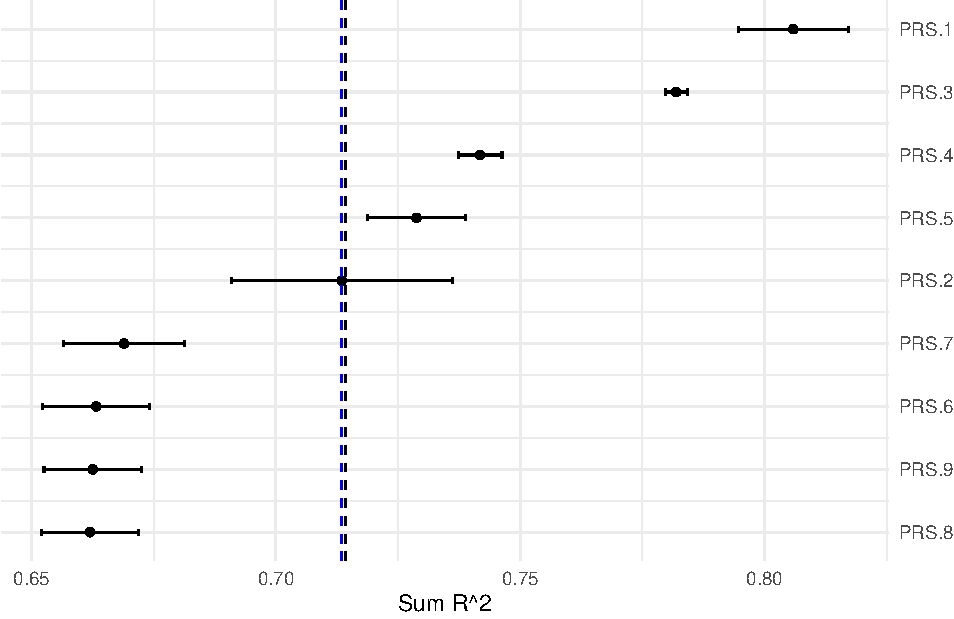
\includegraphics{WorkingExample3_code_files/figure-latex/unnamed-chunk-5-1.pdf}

According to the obtained results, first PRS.1 is selected to analyze
its association with the Trait.

\hypertarget{which-model-of-all-the-possible-ones-should-be-used}{%
\subsection{3. Which model, of all the possible ones, should be
used?}\label{which-model-of-all-the-possible-ones-should-be-used}}

The following figure represents the scatter plot of Trait versus PRS.1
separated by Sex and Diagnostic groups.

\begin{Shaded}
\begin{Highlighting}[]
\FunctionTok{ggplot}\NormalTok{(dat, }\FunctionTok{aes}\NormalTok{(}\AttributeTok{x=}\NormalTok{PRS}\FloatTok{.1}\NormalTok{, }\AttributeTok{y=}\NormalTok{Trait)) }\SpecialCharTok{+}
  \FunctionTok{geom\_point}\NormalTok{() }\SpecialCharTok{+}
  \FunctionTok{geom\_smooth}\NormalTok{(}\AttributeTok{method=}\NormalTok{lm, }\AttributeTok{se=}\ConstantTok{FALSE}\NormalTok{)}\SpecialCharTok{+}
  \FunctionTok{facet\_grid}\NormalTok{(Sex }\SpecialCharTok{\textasciitilde{}}\NormalTok{ Diagnostic, }\AttributeTok{labeller=}\NormalTok{label\_both)}
\end{Highlighting}
\end{Shaded}

\begin{verbatim}
## `geom_smooth()` using formula = 'y ~ x'
\end{verbatim}

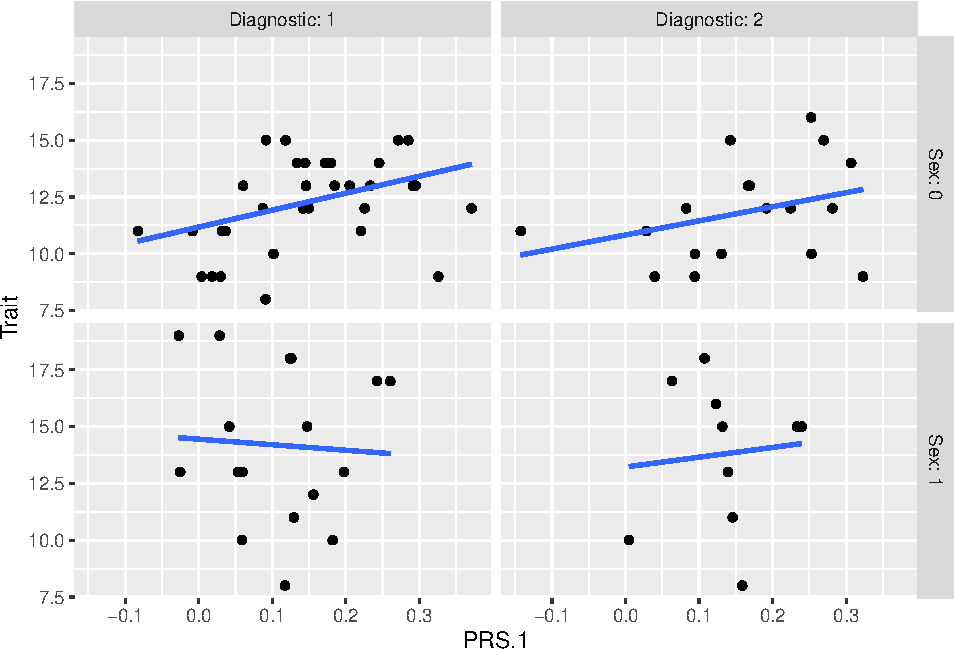
\includegraphics{WorkingExample3_code_files/figure-latex/unnamed-chunk-6-1.pdf}

The plots suggest that the interaction between the PRS.1 and sex is
relevant. Thus, we set the full model candidate (FM):
\(Trait \sim PRS + Sex + Diagnostic + PRS\cdot Sex + PC1 +PC2\).

\hypertarget{for-a-continuous-trait-what-steps-should-be-followed-for-a-correct-analysis}{%
\subsubsection{4. For a continuous trait, what steps should be followed
for a correct
analysis?}\label{for-a-continuous-trait-what-steps-should-be-followed-for-a-correct-analysis}}

\begin{itemize}
\tightlist
\item
  \textbf{4.1. How is the candidate model validated?}
\end{itemize}

First, we validate the normality of the errors and the constant variance
conditions (see the figures and the results of Shapiro test and Levene
test).

\begin{Shaded}
\begin{Highlighting}[]
\CommentTok{\#model}
\NormalTok{FM }\OtherTok{\textless{}{-}} \FunctionTok{lm}\NormalTok{(Trait }\SpecialCharTok{\textasciitilde{}}\NormalTok{ PRS}\FloatTok{.1}\SpecialCharTok{*}\NormalTok{Sex }\SpecialCharTok{+}\NormalTok{ Diagnostic }\SpecialCharTok{+}\NormalTok{ Age }\SpecialCharTok{+}\NormalTok{ PC1 }\SpecialCharTok{+}\NormalTok{ PC2, }\AttributeTok{data=}\NormalTok{dat)}
\CommentTok{\#qq{-}plot for normality }
\FunctionTok{plot}\NormalTok{(FM,}\DecValTok{2}\NormalTok{)   }
\end{Highlighting}
\end{Shaded}

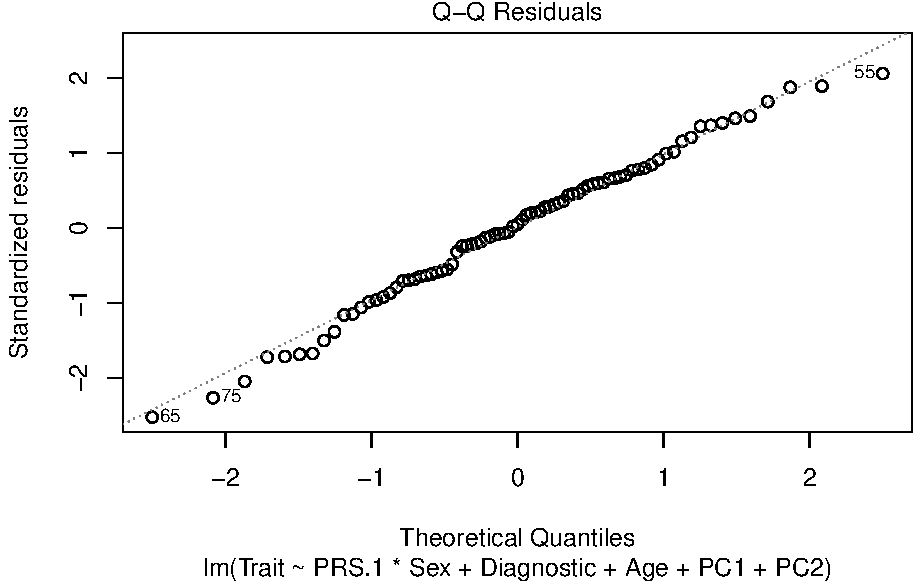
\includegraphics{WorkingExample3_code_files/figure-latex/unnamed-chunk-7-1.pdf}

\begin{Shaded}
\begin{Highlighting}[]
\CommentTok{\#Shapiro{-}Wilk test}
\FunctionTok{shapiro.test}\NormalTok{(FM}\SpecialCharTok{$}\NormalTok{residuals)}
\end{Highlighting}
\end{Shaded}

\begin{verbatim}
## 
##  Shapiro-Wilk normality test
## 
## data:  FM$residuals
## W = 0.98615, p-value = 0.5353
\end{verbatim}

\begin{Shaded}
\begin{Highlighting}[]
\CommentTok{\#plot for variances}
\NormalTok{d }\OtherTok{\textless{}{-}} \FunctionTok{fortify}\NormalTok{(FM)}
\FunctionTok{ggplot}\NormalTok{(d,}\FunctionTok{aes}\NormalTok{(}\AttributeTok{x=}\NormalTok{.fitted, }\AttributeTok{y=}\NormalTok{.stdresid, }\AttributeTok{colour=}\NormalTok{Sex)) }\SpecialCharTok{+} 
  \FunctionTok{geom\_point}\NormalTok{() }\SpecialCharTok{+} 
  \FunctionTok{geom\_hline}\NormalTok{(}\AttributeTok{yintercept=}\DecValTok{0}\NormalTok{, }\AttributeTok{col=}\StringTok{"red"}\NormalTok{)}\SpecialCharTok{+}
  \FunctionTok{facet\_wrap}\NormalTok{(.}\SpecialCharTok{\textasciitilde{}}\NormalTok{Sex)}
\end{Highlighting}
\end{Shaded}

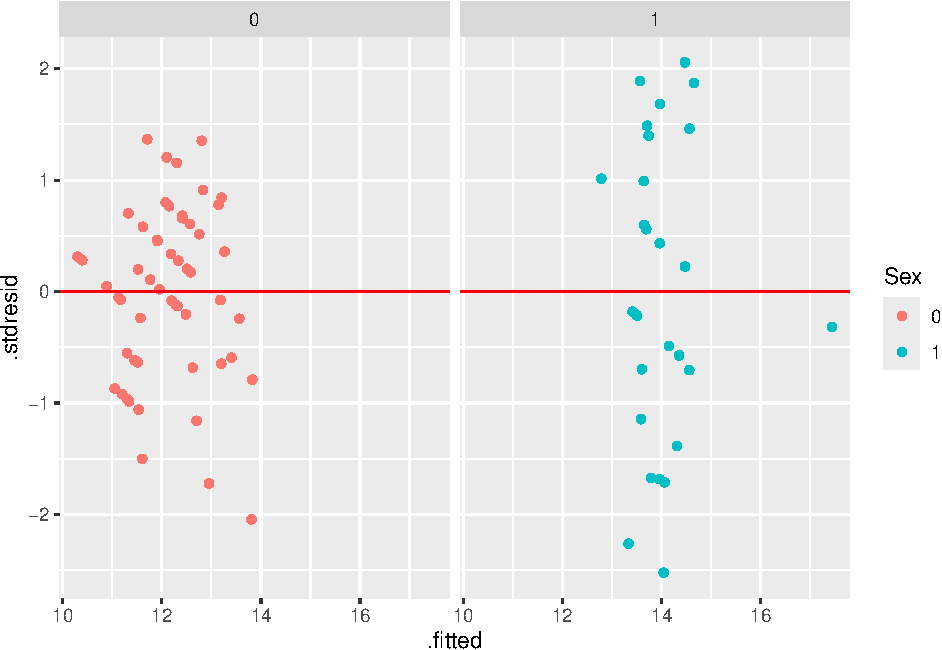
\includegraphics{WorkingExample3_code_files/figure-latex/unnamed-chunk-9-1.pdf}

\begin{Shaded}
\begin{Highlighting}[]
\CommentTok{\#Levene\textquotesingle{}s test}
\FunctionTok{leveneTest}\NormalTok{(.stdresid }\SpecialCharTok{\textasciitilde{}}\NormalTok{ Sex, }\AttributeTok{data=}\NormalTok{d)}
\end{Highlighting}
\end{Shaded}

\begin{verbatim}
## Levene's Test for Homogeneity of Variance (center = median)
##       Df F value    Pr(>F)    
## group  1  15.673 0.0001636 ***
##       79                      
## ---
## Signif. codes:  0 '***' 0.001 '**' 0.01 '*' 0.05 '.' 0.1 ' ' 1
\end{verbatim}

It seems that homocedasticity does not hold.

\begin{itemize}
\tightlist
\item
  \textbf{4.2. What can be done if any validation condition fails?}
\end{itemize}

We have two approaches to assess the possible association with PRS.1 and
the Trait: try a Box-Cox transformation or perform a weighted
permutation test.

First, we try a Box-Cox transformation of the dependent variable: -
Determine the lambda value.

\begin{Shaded}
\begin{Highlighting}[]
\NormalTok{b }\OtherTok{\textless{}{-}} \FunctionTok{boxcox}\NormalTok{(FM)}
\end{Highlighting}
\end{Shaded}

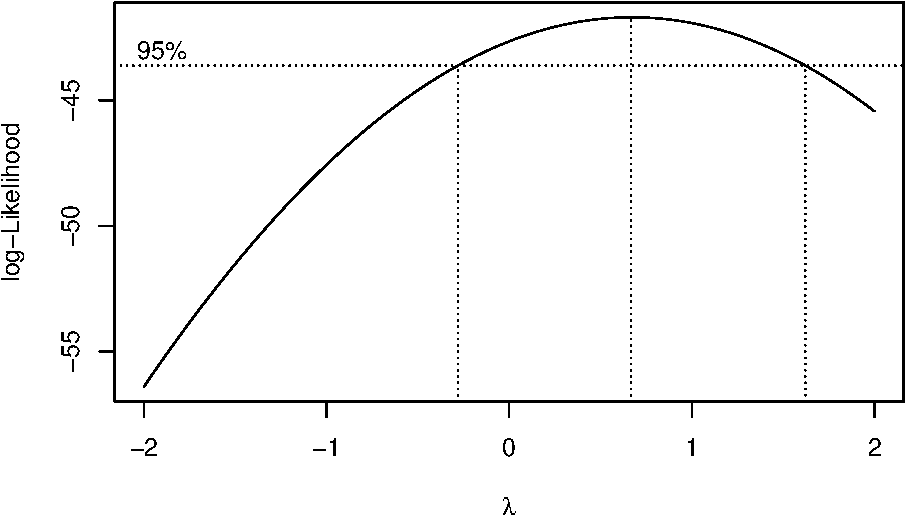
\includegraphics{WorkingExample3_code_files/figure-latex/unnamed-chunk-11-1.pdf}

\begin{Shaded}
\begin{Highlighting}[]
\CommentTok{\# Exact lambda}
\NormalTok{lambda }\OtherTok{\textless{}{-}}\NormalTok{ b}\SpecialCharTok{$}\NormalTok{x[}\FunctionTok{which.max}\NormalTok{(b}\SpecialCharTok{$}\NormalTok{y)]}
\NormalTok{lambda}
\end{Highlighting}
\end{Shaded}

\begin{verbatim}
## [1] 0.6666667
\end{verbatim}

\begin{itemize}
\tightlist
\item
  Transform the dependent variable and establish the new model.
\end{itemize}

\begin{Shaded}
\begin{Highlighting}[]
\NormalTok{dat}\SpecialCharTok{$}\NormalTok{newTrait }\OtherTok{\textless{}{-}}\NormalTok{ (dat}\SpecialCharTok{$}\NormalTok{Trait }\SpecialCharTok{\^{}}\NormalTok{ lambda }\SpecialCharTok{{-}} \DecValTok{1}\NormalTok{) }\SpecialCharTok{/}\NormalTok{ lambda}
\NormalTok{FM }\OtherTok{\textless{}{-}} \FunctionTok{lm}\NormalTok{(newTrait }\SpecialCharTok{\textasciitilde{}}\NormalTok{ PRS}\FloatTok{.1}\SpecialCharTok{*}\NormalTok{Sex }\SpecialCharTok{+}\NormalTok{ Diagnostic }\SpecialCharTok{+}\NormalTok{ Age }\SpecialCharTok{+}\NormalTok{ PC1 }\SpecialCharTok{+}\NormalTok{ PC2, }\AttributeTok{data=}\NormalTok{dat)}
\end{Highlighting}
\end{Shaded}

\begin{itemize}
\tightlist
\item
  Check the normality and homocedasticity conditions.
\end{itemize}

\begin{Shaded}
\begin{Highlighting}[]
\CommentTok{\#Shapiro{-}Wilk test}
\FunctionTok{shapiro.test}\NormalTok{(FM}\SpecialCharTok{$}\NormalTok{residuals)}
\end{Highlighting}
\end{Shaded}

\begin{verbatim}
## 
##  Shapiro-Wilk normality test
## 
## data:  FM$residuals
## W = 0.98029, p-value = 0.2465
\end{verbatim}

\begin{Shaded}
\begin{Highlighting}[]
\CommentTok{\#Levene\textquotesingle{}s test}
\NormalTok{d }\OtherTok{\textless{}{-}} \FunctionTok{fortify}\NormalTok{(FM)}
\FunctionTok{leveneTest}\NormalTok{(.stdresid }\SpecialCharTok{\textasciitilde{}}\NormalTok{ Sex, }\AttributeTok{data=}\NormalTok{d)}
\end{Highlighting}
\end{Shaded}

\begin{verbatim}
## Levene's Test for Homogeneity of Variance (center = median)
##       Df F value    Pr(>F)    
## group  1  13.368 0.0004595 ***
##       79                      
## ---
## Signif. codes:  0 '***' 0.001 '**' 0.01 '*' 0.05 '.' 0.1 ' ' 1
\end{verbatim}

In this case, the suggested Box-Cox transformation with
\(\lambda = 0.667\) does not solve the heteroscedasticity problem. For
this reason we perform a weighted-permutation test.

\begin{Shaded}
\begin{Highlighting}[]
\NormalTok{NM }\OtherTok{\textless{}{-}} \FunctionTok{lm}\NormalTok{(Trait }\SpecialCharTok{\textasciitilde{}}\NormalTok{ Sex }\SpecialCharTok{+}\NormalTok{ Diagnostic }\SpecialCharTok{+}\NormalTok{ Age }\SpecialCharTok{+}\NormalTok{ PC1}\SpecialCharTok{+}\NormalTok{PC2, }\AttributeTok{data=}\NormalTok{dat)}
\NormalTok{FM }\OtherTok{\textless{}{-}} \FunctionTok{lm}\NormalTok{(Trait }\SpecialCharTok{\textasciitilde{}}\NormalTok{ PRS}\FloatTok{.1}\SpecialCharTok{*}\NormalTok{Sex }\SpecialCharTok{+}\NormalTok{ Diagnostic }\SpecialCharTok{+}\NormalTok{ Age }\SpecialCharTok{+}\NormalTok{ PC1}\SpecialCharTok{+}\NormalTok{PC2, }\AttributeTok{data=}\NormalTok{dat)}
\NormalTok{outperm }\OtherTok{\textless{}{-}} \FunctionTok{dR2}\NormalTok{(}\AttributeTok{NullModel=}\NormalTok{NM, }\AttributeTok{FullModel=}\NormalTok{FM, }\AttributeTok{B=}\DecValTok{1000}\NormalTok{, }\AttributeTok{seed=}\DecValTok{165}\NormalTok{,  }\AttributeTok{weights=}\ConstantTok{TRUE}\NormalTok{)}
\NormalTok{outperm}
\end{Highlighting}
\end{Shaded}

\begin{verbatim}
## $dR2
## [1] 0.09217286
## 
## $pvalue
## [1] 0
\end{verbatim}

We observe an increase of 0.092 in the coefficient of determination when
the PRS.1 is included in the model and the permutation test indicates it
is significant.

\begin{itemize}
\tightlist
\item
  \textbf{Last step: We move to the next PRS.}
\end{itemize}

\end{document}
